% possible options for type:
%  da = Diplomarbeit
%  gb = Großer Beleg
%  ms = Master's Thesis
%  bs = Bachelor's Thesis
% possible options for language:
%  english, german, ngerman
% default is: \documentclass[da,ngerman]{stthesis}
\documentclass[ms, english]{stthesis}

% * use this package if you don't want to use a layout based on the offical corporate design from TU Dresden
% * use the given parameter if you only want the title page to be set in TU Dresden layout
%\usepackage[titlepageonly]{tudlayout}

% only used for exemplary lorem ipsum text
\usepackage{lipsum}
\usepackage{todonotes}
\usepackage{pdfpages} % to insert a task description.
%\usepackage[notes,backend=biber]{biblatex-chicago}
%\bibliography{content/bibliography.bib}


% Define the title of the thesis
\title{From Parameter Tuning to Dynamic Heuristic Selection}
% Specify the author of the thesis
\author{Yevhenii Semendiak}
% Specify the date on which the thesis is handed in
\date{\today}
% Specify the birthday of the thesis submitter
\birthday{07.02.1995}
% Specify the place of birth
\birthplace{Izyaslav}
% Specify the name of the supervisor
% Use '\newline' to separate multiple supervisors from each other
\supervisor{MSc. Dmytro Pukhkaiev \newline Dr.-Ing. Sebastian Götz}
% Optionally, you can also use \hsl to define the name of the supervising professor if this is necessary. 
% This defaults to Prof. Aßmann

\newcommand{\todor}[1]{\todo[color=green,inline,size=\small]{Reviewer: #1}}
\newcommand{\todoy}[1]{\todo[color=yellow,inline,size=\small]{Yevhenii: #1}}

% usefull links
% % https://writingcenter.fas.harvard.edu/pages/developing-thesis

\begin{document}
  \maketitle % This sets the title page
  
  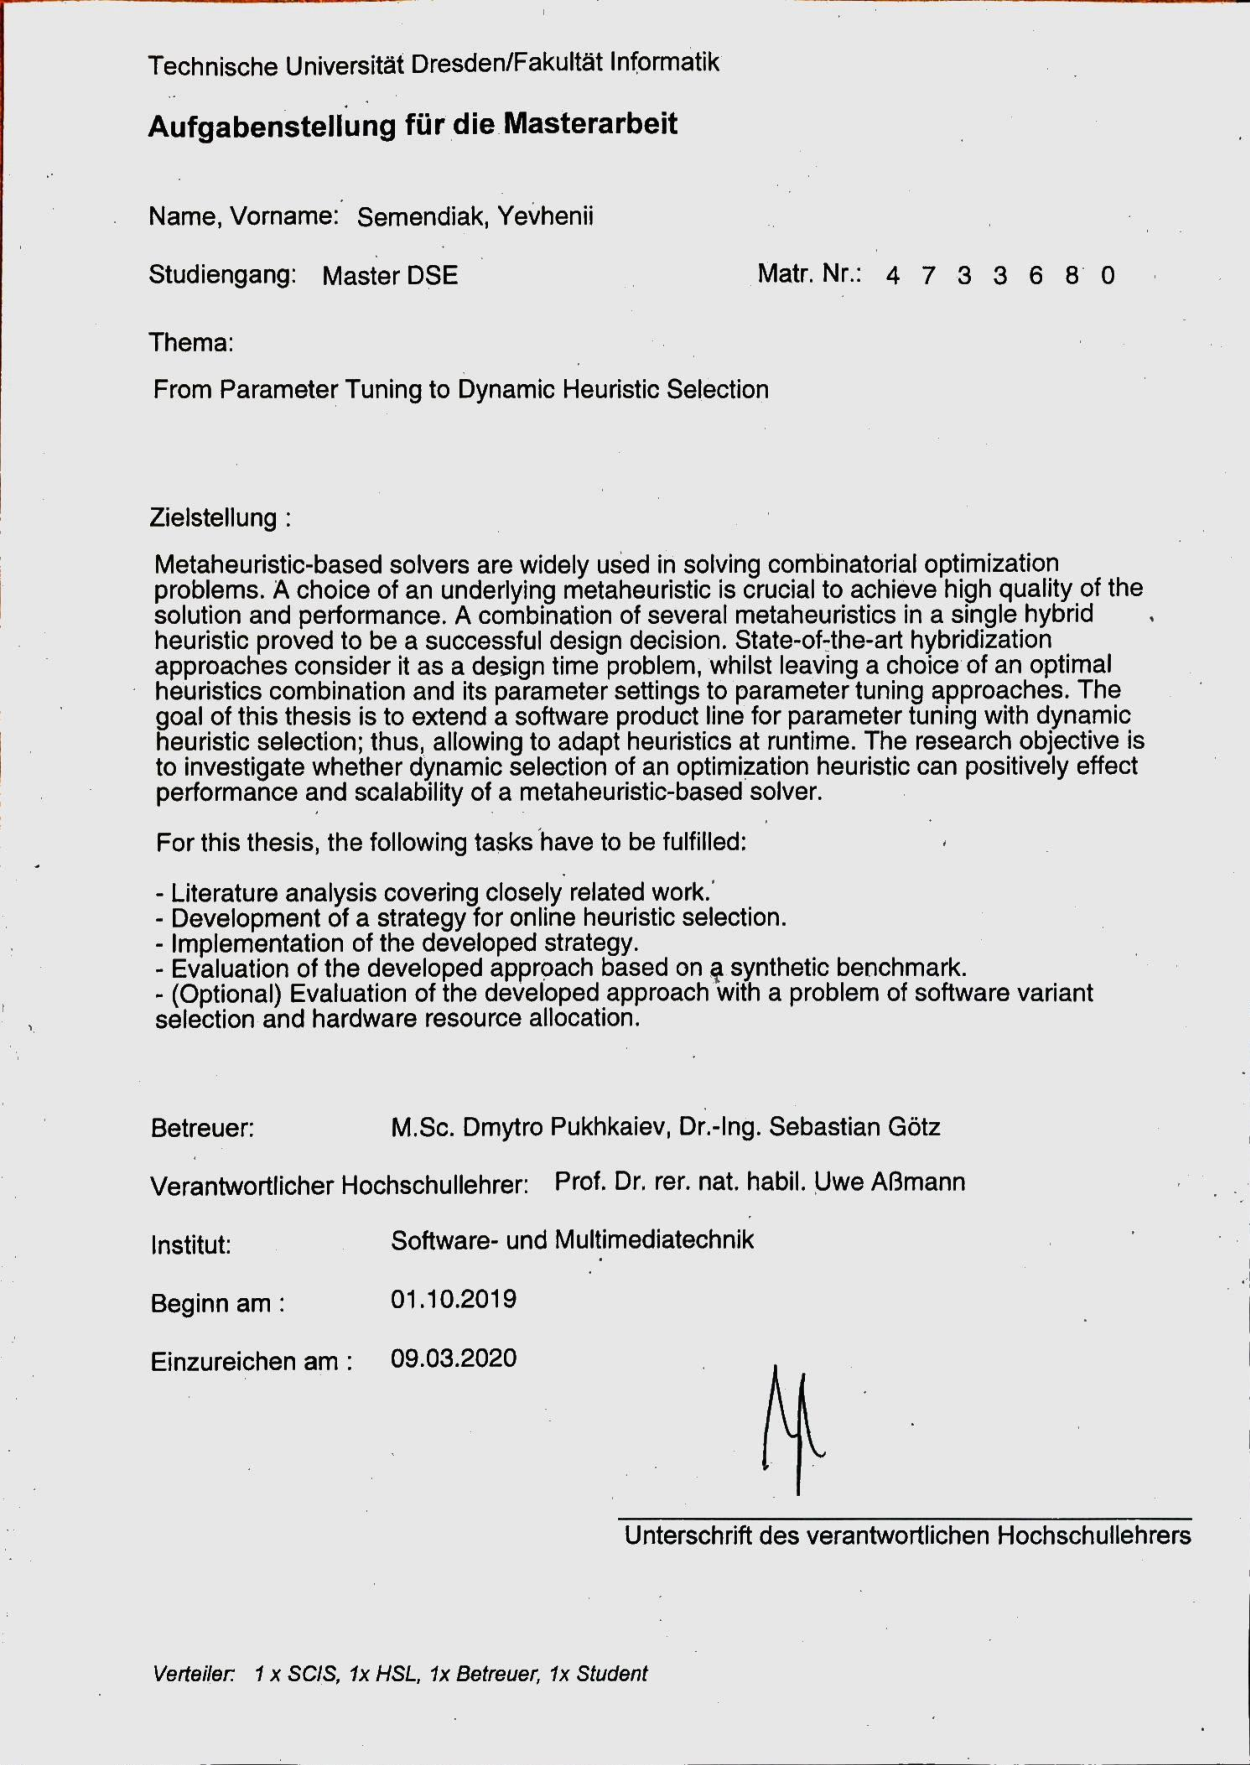
\includepdf{taskDescription.pdf}

  \section*{\vfill{} \thispagestyle{empty}
Statement of Authorship}

I hereby certify that I have authored this Master Thesis entitled “From Parameter Tuning to Dynamic Heuristic Selection“ independently and without undue assistance from third parties. No other than the resources and references indicated in this thesis have been used. I have marked both literal and accordingly adopted quotations as such. There were no additional persons involved in the preparation of the present thesis. I am aware that violations of this declaration may lead to subsequent withdrawal of the degree.
\bigskip{}

\noindent Dresden, \today %\today % if you defined date earlier
\vspace{2.5cm}

\noindent Yevhenii Semendiak \cleardoublepage{}
\todoy{should I add a disclaimer like this?}
  
  \tableofcontents
  
  \newpage
\section*{Abstract}
The importance of balance between exploration and exploitation plays a crucial role while solving combinatorial optimization problems. This balance is reached by two general techniques: by using an appropriate problem solver and by setting its proper parameters. Both problems were widely studied in the past and the research process continues up until now. The latest studies in the field of automated machine learning propose merging both problems, solving them at design time and later strengthening the results at runtime. To the best of our knowledge, the \emph{generalized} approach for solving the parameter setting problem in heuristic solvers has not yet been proposed. Therefore, the concept of merging heuristic selection and parameter control has not been introduced.

In this thesis we propose an approach for generic parameter control in meta-heuristics by means of reinforcement learning (RL). Making a step further, we suggest a technique for merging the heuristic selection and parameter control problems and solving them at runtime using RL-based hyper-heuristic. The evaluation of the proposed parameter control technique on a symmetric traveling salesman problem (TSP) revealed its applicability by reaching the performance of tuned in offline and used in isolation underlying meta-heuristic. Our approach provides the results on par with the best underlying heuristics with tuned parameters.

  \chapter{Introduction}\label{intro}

\section{Motivation}
Heuristic-based optimization is a popular research area~\cite{junger2003combinatorial,biegler2004retrospective,festa2014brief}. Numbers of optimization problems are defined, but an ideal approach for their struggling does not exist. This issue was formalized by the \emph{no-free-lunch theorem for optimization} (NFLT)~\cite{wolpert1997no}, which states that ``all search algorithms have the same average performance over all possible optimization problems''. Heuristic solver acts by means of \emph{exploration} (effort diversification over a search space) and \emph{exploitation} (effort intensification on a promising area) operations. The success of heuristic on the problem at hand is defined by the exposed strength of both operations (E\&E) and the provided balance between them (EvE).

Firstly, one could try to set proper values of hyper-parameters, exposed by the algorithm. This process is formalized under the notion of \emph{parameter settings problem} (PSP), whose resolution can be done before running the algorithm (design time), or while it solves the OP (runtime). The former approach is also called \emph{parameter tuning} and can be tackled by numerous universal tuning systems ~\cite{hutter2009paramils,hutter2011sequential,lopez2016irace,falkner2018bohb,brise2spl}. A key assumption of this software is an expensiveness of the target system evaluation in terms of computational resources. Expensiveness is tackled creating a surrogate learning model, which simulates direct evaluations. The latter approach \emph{parameter control} was originally introduced for evolutionary algorithms~\cite{karafotias2014parameter} and nowadays appears in an \emph{algorithm-dependent} manner. However, even a proper parameter setting may not lead to the best results for the problem at hand. 

The second way for reaching the EvE balance is a proper algorithm selection. It resolves the direct consequence of NFLT by searching appropriate solver for problem at hand and was formalized as the \emph{algorithm selection problem} (ASP). Hyper-heuristics are commonly used for solving ASPs. They may perform low-level heuristic selection before solving the actual problem, or at runtime~\cite{burke2019classification}. To operate on-line, hyper-heuristics often utilize reinforcement learning (RL) techniques~\cite{moriarty1999evolutionary,mcclymont2011markov}, while for design time, a regular parameter tuning could be used.

The research is not at a standstill and nowadays the researchers are actively attempting to merge ASP and PSP into the united \emph{algorithm selection and parameter setting problem} (APSP). For instance, in automatic machine learning such combination was formalized as the \emph{combined algorithm selection and hyper-parameter optimization} problem (CASH)~\cite{thornton2013auto}, while for heuristics the explicit studies of APSP merging and solving at runtime were not found. To tackle ML CASH problem several frameworks based on the existing parameter tuning systems were created~\cite{thornton2013auto,feurer2015efficient,olson2019tpot}. However, those solutions are not applicable in case of heuristics, since they are (1) purely related to ML field and (2) acting at design time due to ML techniques nature. One may follow the ML approach of the united APSP search space definition and solving for heuristics, but it is applicable \emph{only} at design time. However, when it comes to runtime, it turns out that the universal technique for setting the parameters on-line (parameter control) in heuristics has not yet been proposed. It is essential, since this (PSP) is one of two required methodologies for solving heuristic APSP at runtime. The other building block (ASP) is already available in on-line hyper-heuristics.

\section{Research objective}\label{intro: research objective}
The goal of this thesis is to basing on the existing parameter tuning software, propose an \emph{on-line} approach for solving \emph{both} PSP and ASP problems for heuristic solvers.

In order to fulfill the goal defined above, the following \textbf{research questions} should be answered:
\begin{itemize}
	\item \textbf{RQ1} Is it possible to perform the algorithm configuration at runtime on a generic level?
	
	\item \textbf{RQ2} Is it possible to simultaneously perform algorithm selection and parameters adaptation while solving an optimization problem?
	
	\item \textbf{RQ3} What is the effect of selecting and adapting algorithm while solving an optimization problem?
\end{itemize}


\section{Solution overview}
In this thesis we propose the unification of both ASP and PSP into a single problem. In order to do so, we firstly introduce a generic runtime PSP solution; secondly, we suggest joining several PSPs search spaces into a united APSP.

To overcome the sparseness issue we propose a complex solution, which is spread in both search space structure and prediction process. For the APSP representation we suggest using of a data structure, similar to feature trees from software product lines field. Doing so we treat a solver type and its hyper-parameters uniformly as a regular parameter in a search space. The dependencies between parameters are explicitly handled in form of a parent-child relationship. As a result, the search space could be viewed as a layered structure, where on the first level remains (categorical) parameter defining the algorithm type, and on the level(s) below its respective hyper-parameters (categorical and numerical). The prediction process is made sequentially for each level, utilizing the available performance evidences in form of already tried configurations in this optimization session. Therefore, in the united APSP we firstly build a surrogate model for the algorithm type prediction. Afterwards, when the solver type is selected, we filter the performance evidences to operate on data, which is relevant to the selected algorithm type. With this filtered data we build a surrogate for the second level and predict the selected algorithm parameters. Dependencies among algorithm-related parameters are also treated in form of the parent-child relationship, therefore, we proceed the level-wise prediction process until obtaining a completed configuration. Next, we continue solving the underlying OP with the defined algorithm type and its parameters to obtain new evidence and repeat configuration prediction process. This reinforcement learning techniques enables us to solve the APSP on-line, while iteratively tackling the OP at hand. 

The structure of this thesis is organized as follows. Firstly, in \cref{bg} we refresh the reader's background knowledge in the field of optimization problems and solver types, focusing on heuristics. We also review the parameter setting and the available solutions for this problem. In \cref{Concept description} one will find a description of the proposed approach for generic parameter control and APSP problem unification. There we also present both structural and functional requirements for system components. \cref{impl} is dedicated to the review of implementation details, including a code basis selection, aforementioned requirements realization and the developed system workflow representation. We evaluate the proposed concept and discuss the results in \cref{eval}. \cref{conclusion} concludes the thesis and \cref{future work} describes the future work.

  
  \chapter{Background}\label{bg}
\todor{add important terminology for parameter tuning}
one-two sentence definition of 
\begin{itemize}
  \item Heuristic
  \item Meta-heuristic
  \item Hybrid-heuristic
  \item Hyper-heuristic
\end{itemize}

\section{Meta-heuristics}
\subsection{Classification}

- from the solution point of view (construction / perturbation)

- solution availability (any-time / till the end)
     
\subsection{Related meta-heuristics description}
\todor{what does related mean? why did you choose exactly these 3(4) heuristics to be described? is there sth special the reader should know about them?}
- GA

- SA

- ES

- would be cool to add VNS
  
\section{Hybrid meta-heuristics and hyper-heuristics}
\subsection{Classification of hyper-heuristics}
- heuristic selection

- heuristic generation

- on-line learning hyper-heuristics

- off-line learning hyper-heuristics

- no-learning hyper-heuristics


\section{Scope of work defined}
\todor{consider emphasizing the problem here. show, how do these algorithm perform with the problem you try to solve. Save a detailed explanation of TSP, etc. for later. But make a vivid example why single MHs are under-performing.}
- on-line selection out of GA, SA, ES, parameter optimization to solve defined problem
\todor{shouldn't you first introduce parameter optimization to make such a conclusion?}

  
  \chapter{Related work}\label{relwork}
\todor{what is the goal of this chapter? it should not be just an enumeration of approaches} 
utilize surveys 
\todoy{Broad survey \cite{surv:kerschke2019automated}, Online algorithm selection at page 27}
\todoy{\cite{surv:drake2019recent}}


Previously reviewed systems that could be refereed in Related Work: 
\section{AUTO-SKLEARN}
- CASH (Combined Algorithm Selection and Hyperparameter optimization) problem
- pros and cons (on-line or off-line, problems to solve, extensibility)
- \cite{autosklearn:feurer2015efficient}

\section{BOHB}
- possible to try, but model will be lost in 'holes' of search space (no tree structure)
- should i cite it at all? (probably, it is not really relevant, since BOHB - Robust and Efficient Hyperparameter Optimization at Scale)

\section{IRACE}
- approach \cite{irace:lopez2016irace}
- off-line tuning
- is it really relevant?

\todor{BRISE?}

  
  \chapter{Concept description}
\paragraph{In this chapter} we describe the concept of developed selection Hyper~-Heuristic with parameter control, not diving deep into the implementation details.
The best practice in software engineering is to minimize an effort for the implementation and reuse already existing, well-tested and broadly used code.
With this idea in mind we had decided to use one of previously created (and highlighted by us in \ref{bg: parameter tuning}}) hyper~-parameter tuning systems as the code basis and those turn it into the core of hyper~-heuristic.
We also reuse the set of already developed heuristics as the Low Level Heuristics for designed Hyper~-Heuristic.

The structure of this chapter is as follows.
First, we define the Search Space entity in \ref{concept:search space}, it requirements and structure. 
It should bound the world of Low Level Heuristics and the world of Hyper~-parameters of those heuristics.


Second, we describe the Prediction process within the previously defined Search Space in \ref{concept:prediction}.
Here we highlight an importance of a prediction model decoupling from the previously defined Search Space structure.
Doing so, we provide certain level of flexibility for user in the usage of different prediction models or developing his own.


Third, in \ref{concept:llh} we gather our attention onto the Low Level Heuristics - a working horse of the hyper~-heuristic.
Here we highlight the requirements for LLH in terms of features that will be used by HH.


Later, we select the code basis. We analyze the existing systems and highlight important non-functional characteristics for \ref{concept:code basis selection} hyper~-heuristic and \ref{concept:llh code basis selection} low level heuristics set.


Finally, in \ref{concept:changes analysis} we conclude this chapter with the analysis of required changes, that are needed to be accomplished for turning code base system into the hyper~-heuristic.


\section{Search Space}\label{concept:search space}
\paragraph{Importance explanation}
\paragraph{Required structure} feature-tree structured



\section{Prediction process}\label{concept:prediction}
\paragraph{Importance explanation}
\paragraph{Requirements} generality, top-down approach of optimization
-- different views of same Configuration (level-dependent) - filtering, transformation
-- consider problem features? while selecting meta-heuristic \cite{surv:kerschke2019automated} page 6


\section{Low Level Heuristics}\label{concept:llh}
\paragraph{Importance explanation}
\paragraph{Requirements}



\section{Code basis selection}
With the aim of effort reuse, the code base should be selected for implementation of the designed hyper~-heuristic approach.

\subsection{Hyper~-Heuristics Code Base}\label{concept:hh code basis selection}
A.k.a. "brain". Need to find a better way to call this part of HH..
\subsubsection{Requirements}
\subsubsection{Parameter tuning frameworks}
\paragraph{SMAC}
\paragraph{BOHB}
\paragraph{IRACE}
\paragraph{BRISEv2}
\todoy{Maybe, smth else..}
\subsubsection{Conclusion}
BRISEv2 is the best system for code basis.

\subsection{Low Level Heuristics}\label{concept:llh code basis selection}
\subsubsection{Requirements}
\subsubsection{Heuristic frameworks}
\paragraph{SOLID}
\paragraph{MLRose}
\paragraph{OR-tools}
\paragraph{pyTSP}
\paragraph{LocalSolver}
\paragraph{jMetalPy}

\subsubsection{Conclusion}
jMetalPy is cool!


\section{Scope of Required Changes}\label{concept:changes analysis}

\subsection{Search Space} highlight - should be done in feature-tree structured search space
\subsubsection{Current state description} What is the problem with the current Search Space?
\subsubsection{Scope of work analysis:} throw away and write a new one :D

\subsection{Prediction Process} highlight - should be done in feature-tree structured search space
\subsubsection{Description of current state}
\subsubsection{Heterogeneous data?} short description of data preprocessing
\subsubsection{Scope of work analysis} 

\subsection{Low Level Heuristics}
\subsubsection{Description of current state}
\subsubsection{Scope of work analysis}

\subsection{Conclusion?}
we selected BRISEv2, jMetalPy because they are cool.
the amount of work is vast so lets dive into it in the next chapter!

  
  \chapter{Implementation}

\section{Analysis of required changes in system}
\subsection{Description of BRISE v2.2.0}

\paragraph{Data preprocessing}

\paragraph{Model compatibilities}
      
\paragraph{Search space compatibilities}

\subsection{Meta-heuristics repository}
-table and short comparison of checked repositories 
% https://docs.google.com/spreadsheets/d/19xjL_ire0R5VLP9seCE5_4sWorSMZP4xvgx7d1q4a9s/edit#gid=0
\begin{itemize}
  \item Solid
  \item mlrose
  \item jMetalPy
  \item or-tools
  \item pyTSP
  \item LocalSolver
\end{itemize}


\subsubsection{jMetalPy in more details}
\paragraph{Available Meta-heuristics}
\paragraph{Required features}
- any-time (or predictable) termination

- warm-startup

\paragraph{opened PR}


\subsection{Development planning}
\paragraph{use-case definition}
\paragraph{generalization with team}
\paragraph{requirements engineering}
- interfaces
\paragraph{class diagrams}
\paragraph{data flow}

  
  \chapter{Evaluation}


\section{Evaluation Plan}

\subsection{Optimization Problems Definition}
\subsubsection{Traveling Salesman Problem}
\paragraph{tsplib95 benchmark set}
which problem I want to solve with hyper-heuristic
$http://comopt.ifi.uni-heidelberg.de/software/TSPLIB95/STSP.html$

\subsection{Hyper-Heuristic Settings}
To evaluate the performance of developed system we first need to compare it with the base line. In our case it is the simple meta-heuristic that is solving the problem with static hyper-parameters.

In order to organize the evaluation plan, we distinguish two stages of setup, where different approaches could be applied. 
At the first stage we select Low Level Heuristic, while at the second one we select hyper-parameters for LLH.
The approaches for each step are represented in table \ref{evaluation: settings table}.

% highlight that such MHs as Simulated Annealing are now "restarting". It measn, that is in SA case, the Temperature parameter change drops to initial state. Thus here we obtain Iterative Simulated Annealing

\begin{table}[h!]
	\centering
	\begin{tabular}{|l|l|}
		\hline
		\textbf{Low Level Heuristics selection} & \textbf{LLH Hyper-parameters selection} \\
		\hline
		1. Random & 1. Default \\
		2. Multi Armed Bandit & 2. Tuned beforehand \\
		3. Sklearn Bayesian Optimization & 3. Random \\
		4. Static selection of SA, GA, ES & 4. Tree Parzen Estimator \\
		& 5. Sklearn Bayesian Optimization\\
		\hline
	\end{tabular}
	
	\caption{System settings for benchmark}
	\label{evaluation: settings table}
\end{table}


For instance, mentioned above baseline could be described as $Settings 4.1.$ for meta-heuristics with default hyper-parameters and as $Settings 4.2.$ for meta-heuristics with tuned beforehand hyper-parameters.

For our benchmark we selected following settings sets:

\begin{itemize}
	\item \textit{Baseline:} $4.1, 4.2;$
	\item \textit{Random Hyper-heuristic:} $1.1, 1.2, 1.3, 4.3;$
	\item \textit{Parameter control:} $4.4, 4.5;$
	\item \textit{Selection Hyper-Heuristic:} $2.1, 3.1, 2.2, 3.2;$
	\item \textit{Selection Hyper-Heuristic with Parameter Control:} $2.4, 2.5, 3.4, 3.5;$
\end{itemize}

The goal of parameter control is to reach the performance of algorithms with the tunned hyper-parameters.
The goal of hyper-heuristic is to reach the performance of the best underlying algorithm.

Each of this settings will be discussed in details in following section.


\subsection{Selected for Evaluation Hyper-Heuristic Settings}
\paragraph{Baseline}

\paragraph{Hyper-heuristic With Random Switching of Low Level Heuristics}

\paragraph{Parameter control}

\paragraph{Selection Only Hyper-Heuristic}

\paragraph{Selection Hyper-Heuristic with Parameter Control}


\section{Results Discussion}

\subsection{Baseline Evaluation}

\paragraph{Meta-Heuristics With Default Hyper-Parameters}

\paragraph{Meta-Heuristics With Tuned Hyper-Parameters}

\paragraph{Results Description and Explanation}


\subsection{Hyper-Heuristic With Random Switching of Low Level Heuristics}

\paragraph{Results Description and Explanation}


\subsection{Parameter Control}

\paragraph{Results Description and Explanation}


\subsection{Selection Only Hyper-Heuristic}
auto-sklearn paper, p.2 - comparison of GP and TPE BOs.

\paragraph{Results Description and Explanation}


\subsection{Selection Hyper-Heuristic with Parameter Control}

\paragraph{Results Description and Explanation}

\section{Conclusion}

  
  \chapter{Conclusion}
\todor{answer research questions}
comparison to HITO~\cite{guizzo2015hyper}
  
  \chapter{Future work}
\paragraph{add more sophisticated models}
\paragraph{dependencies / constraints in search space}
\paragraph{add new class of problem (jmetalpy easly allows it)}
\paragraph{evaluation on different types and classes}
\paragraph{adaptive time for tasks}
\paragraph{bounding LLH by number of evaluations, not time}
\paragraph{interesting direction: apply to automatic machine learning problems solving, compare to auto-sklearn.}
\paragraph{technique to optimize obtained surrogate model should be generalized}
\paragraph{investigate more deeply decoupling of data preprocessing and learning algorithm} auto-sklearn
\paragraph{influence for warm-start onto this kind of HH (by off-line learning)}
Although, the influence of meta-learning, applied in Auto-Sklearn system~\cite{feurer2015efficient} to warm-start the learning mechanism proved to worth the effort spent, as well as it was reported by developers of Selective Hyper-Heuristics with mixed type of learning~\cite{uludaug2013hybrid,}, it is intriguing to check an influence of metal-learning onto Selective Hyper-Heuristics with Parameter Control.

\paragraph{Random Forest HLH surrogate model}
% TODO: try a random forest as a 1ST level of HH, SMAC paper (short version), PAGE 7, CITES 18, 19.

\paragraph{add other learning metrics}
Inspiration could be found at:
- EAs in~\cite{karafotias2014generic}: progress stagnation, 

\todor{consider merging with conclusion, if too short}
  
  \bibliographystyle{IEEEtran}
  \todoy{is it correct style?}
  \todor{better the one with first letters of family names and year}
  \bibliography{content/bibliography.bib}
  %\printbibliography
  
  
  \appendix
  \chapter{Appendix}
  \section{Additional Information}
  
  \section{More Important Information}
  
\end{document}
